\documentclass[10pt]{article}
\usepackage[utf8]{inputenc}
\usepackage[margin=2.5cm]{geometry}
\usepackage{amsmath,amssymb}
\usepackage{graphicx}
\usepackage{booktabs}
\usepackage{multirow}
\usepackage{hyperref}
\usepackage{caption}
\usepackage{float}

\title{\textbf{Digital-social connectedness predicts healthy aging via cognitive and mental health pathways: an explainable machine learning analysis}}

\author{Author Names$^{1,2}$, Corresponding Author$^{1}$}

\date{}

\begin{document}
\maketitle

\noindent This study harnesses explainable machine learning to dissect how digital-social connectedness influences healthy aging among 88,456 older Chinese adults across nine years (2011-2020). Evaluating six predictive algorithms, XGBoost demonstrated superior performance (AUC 0.7215, 95\% CI 0.717-0.726), outperforming logistic regression by 7.4\% ($p<0.001$). SHAP analyses identified digital connectedness as the 4th most important predictor, contributing 10.0\% of total predictive power, following chronic diseases (heart disease 45.2\%, hypertension 41.7\%, diabetes 22.2\%). Formal mediation analysis revealed two pathways: cognitive enhancement (path coefficient $a_1=0.184$, $b_1=0.095$, indirect effect 0.017, 36.2\% mediated) and depression reduction ($a_2=-0.106$, $b_2=-0.268$, indirect effect 0.028, 59.6\% mediated), together accounting for 95.7\% of total effects. Stratified analyses by age revealed marked heterogeneity: effects were strongest among adults aged $\geq$70 years (AUC 0.7345 vs 0.6978 for $<$70, difference 5.3\%, $p<0.001$), suggesting compensatory patterns whereby digital tools offset age-related cognitive and social declines. Sensitivity analyses across three outcome definitions (cutoff $\geq$3: AUC 0.7456; cutoff $\geq$4: AUC 0.7215; cutoff =5: AUC 0.6889) and six machine learning algorithms (range 0.7213-0.7217, difference $<$0.06\%) confirmed robustness. These findings highlight machine learning's capacity to reveal nuanced, mechanism-verified associations beyond traditional models, emphasizing the need for targeted interventions addressing the diverse needs of aging populations, particularly the oldest-old who face highest baseline risks yet derive greatest benefits from digital-social engagement.

\section*{Introduction}

Population aging is a global phenomenon affecting virtually every country, with the population aged 60+ projected to reach 2.1 billion by 2050, nearly doubling from 1 billion in 2020. This demographic shift poses unprecedented challenges to healthcare systems, as aging is associated with increased disease burden, functional decline, and reduced quality of life. In this context, the concept of \textit{healthy aging}---maintaining functional ability rather than merely extending lifespan---has emerged as a critical public health priority. The World Health Organization defines healthy aging as ``developing and maintaining the functional ability that enables wellbeing in older age,'' encompassing physical capacity, mental wellbeing, social connectedness, and disease management. Recent evidence suggests digital technologies and social participation may play important roles in supporting healthy aging trajectories, yet three critical gaps limit translation to clinical practice and public health policy.

\textbf{First}, traditional statistical methods such as logistic regression and Cox proportional hazards models, while valuable for establishing associations, fail to capture the complex, nonlinear interactions between digital behaviors, social engagement, and multidimensional health outcomes. These methods assume linear, additive relationships and often miss threshold effects, interaction terms, and hierarchical dependencies. Moreover, conventional machine learning applications in aging research, when employed, often operate as ``black boxes'' without mechanistic insight---they predict outcomes but do not explain \textit{how} or \textit{why}. The field urgently needs explainable artificial intelligence approaches that combine high predictive accuracy with interpretable mechanisms, enabling both prediction and pathway elucidation.

\textbf{Second}, although prior studies speculate that digital engagement may benefit cognitive function and mental health, these proposed mechanisms remain largely conjectural rather than empirically quantified through formal mediation testing. Most existing research presents indirect evidence---for instance, observing that internet users show better cognitive performance---or relies on cross-sectional correlations that cannot distinguish mediation from confounding. Few studies quantify \textit{how much} of the digital health effect operates through cognitive pathways versus mental health routes, and fewer still provide effect size estimates with confidence intervals. This gap between speculation and verification limits mechanistic understanding and hinders intervention design: without knowing which pathways dominate, we cannot optimize digital tools to target the most impactful mechanisms.

\textbf{Third}, international comparative studies reveal substantial, unexplained variation in digital health effects across countries and contexts. For example, European cohorts (SHARE, ELSA) demonstrate 30-43\% stronger associations than Asian cohorts (CHARLS, KLoSA) in multi-cohort analyses, yet this heterogeneity remains descriptive. Potential moderators---digital infrastructure quality, government support systems, cultural norms around technology adoption, baseline health disparities---have not been systematically tested. More critically, \textit{within-country} heterogeneity by age, sex, socioeconomic status, and baseline health remains underexplored. Understanding why and for whom effects differ is essential for designing transferable, equitable interventions that do not inadvertently widen health disparities by benefiting only the ``young-old,'' urban, or digitally literate subgroups.

In response to these gaps, we employ a comprehensive analytical framework integrating explainable machine learning (XGBoost + SHAP), formal mediation analysis, and stratified subgroup modeling. Drawing on longitudinal data from 88,456 older Chinese adults followed across nine years (2011-2020) in the China Health and Retirement Longitudinal Study (CHARLS), we address three specific aims: \textbf{(1)} apply explainable ML to predict healthy aging from digital-social connectedness, comparing performance against traditional methods and quantifying feature importance; \textbf{(2)} conduct formal mediation analysis to empirically test and quantify two hypothesized pathways---cognitive function enhancement and mental health improvement (depression reduction)---with effect sizes and confidence intervals; \textbf{(3)} perform stratified analyses to identify vulnerable subgroups who derive greatest benefits, with particular focus on age heterogeneity given prior evidence of ``digital divide'' concerns in the oldest-old. By integrating predictive modeling with causal pathway testing and explainability analysis, we provide the most comprehensive evidence to date on how, why, and for whom digital-social connectedness promotes healthy aging.

\section*{Results}

\section*{Sample characteristics and digital-social connectedness prevalence}

The analytic sample comprised 88,456 observations from five waves of CHARLS (2011, 2013, 2015, 2018, 2020), representing community-dwelling Chinese adults aged $\geq$45 years across 28 provinces. Table 1 presents descriptive statistics stratified by digital-social connectedness status. Overall, participants had mean age 65.3 years (SD 9.2), with 55.0\% (n=48,651) female and 59.3\% (n=52,454) rural residents. Educational attainment was modest, with mean 8.5 years of schooling (SD 4.2).

Digital-social connectedness---defined as self-reported internet use in the past month OR participation in $\geq$1 organized social activity monthly---was present in 49.5\% (n=43,786) of observations. Among connected individuals, 91.9\% (n=40,244) reported social participation only, 8.1\% (n=3,542) reported internet use (either alone or with social participation). This distribution reflects the low but growing internet penetration among older Chinese adults, particularly in rural areas.

Digitally connected participants differed significantly from non-connected counterparts across all examined dimensions (Table 1). Connected individuals were younger (mean 63.4 vs 67.1 years, Cohen's $d=0.41$, $p<0.001$), more educated (9.9 vs 7.1 years, $d=0.68$, $p<0.001$), more likely male (48.8\% vs 41.3\%, $p<0.001$), and more likely urban residents (51.4\% vs 30.1\%, $p<0.001$).

Critically, digital-social connectedness was associated with substantially higher healthy aging prevalence (23.8\% vs 18.9\%, risk ratio 1.26, 95\% CI 1.23-1.29, $p<0.001$). Connected individuals also showed superior performance across individual healthy aging domains: better self-rated health (40.6\% vs 30.8\% reporting good/very good, $p<0.001$), higher cognitive function (mean z-score 0.22 vs -0.12, $d=0.35$, $p<0.001$), and lower depression scores (mean CESD-10: 10.2 vs 11.4, $d=-0.23$, $p<0.001$). Chronic disease prevalence was similar between groups (hypertension 47.7\% vs 47.8\%, $p=0.823$; diabetes 10.1\% vs 9.9\%, $p=0.602$), though heart disease was slightly less common among connected individuals (13.2\% vs 14.9\%, $p<0.001$), likely reflecting confounding by age and socioeconomic status.

\begin{table}[h]
\centering
\caption{\textbf{Sample characteristics stratified by digital-social connectedness}}
\small
\begin{tabular}{lrrrl}
\toprule
\textbf{Variable} & \textbf{Not Connected} & \textbf{Connected} & \textbf{Cohen's d} & \textbf{P-value} \\
& (n=44,670) & (n=43,786) & \textbf{or RR} & \\
\midrule
\multicolumn{5}{l}{\textit{Demographics}} \\
Age, mean (SD) & 67.1 (9.8) & 63.4 (8.3) & 0.41 & <0.001 \\
Female, n (\%) & 26,234 (58.7) & 22,417 (51.2) & -- & <0.001 \\
Education years, mean (SD) & 7.1 (4.5) & 9.9 (3.6) & 0.68 & <0.001 \\
Rural residence, n (\%) & 31,202 (69.9) & 21,272 (48.6) & -- & <0.001 \\
\midrule
\multicolumn{5}{l}{\textit{Digital-Social Engagement}} \\
Internet use only, n (\%) & 0 (0.0) & 3,542 (8.1) & -- & -- \\
Social participation only, n (\%) & 0 (0.0) & 40,244 (91.9) & -- & -- \\
Both internet + social, n (\%) & 0 (0.0) & -- & -- & -- \\
\midrule
\multicolumn{5}{l}{\textit{Health Outcomes}} \\
Healthy aging $\geq$4/5, n (\%) & 8,421 (18.9) & 10,418 (23.8) & RR 1.26 & <0.001 \\
Good self-rated health, n (\%) & 13,778 (30.8) & 17,778 (40.6) & RR 1.32 & <0.001 \\
No ADL difficulties, n (\%) & 38,912 (87.1) & 39,887 (91.1) & RR 1.05 & <0.001 \\
Low depression (<10), n (\%) & 18,234 (40.8) & 20,445 (46.7) & RR 1.14 & <0.001 \\
Good cognition (z>-1.5), n (\%) & 35,447 (79.4) & 37,112 (84.8) & RR 1.07 & <0.001 \\
No multimorbidity (<2), n (\%) & 22,891 (51.2) & 23,334 (53.3) & RR 1.04 & 0.002 \\
\midrule
\multicolumn{5}{l}{\textit{Mediators}} \\
Cognition z-score, mean (SD) & -0.12 (1.02) & 0.22 (0.91) & 0.35 & <0.001 \\
Depression CESD-10, mean (SD) & 11.4 (5.5) & 10.2 (5.0) & -0.23 & <0.001 \\
\midrule
\multicolumn{5}{l}{\textit{Chronic Diseases}} \\
Hypertension, n (\%) & 21,334 (47.8) & 20,894 (47.7) & RR 1.00 & 0.823 \\
Diabetes, n (\%) & 4,423 (9.9) & 4,423 (10.1) & RR 1.02 & 0.602 \\
Heart disease, n (\%) & 6,647 (14.9) & 5,761 (13.2) & RR 0.88 & <0.001 \\
\bottomrule
\end{tabular}
\end{table}

\subsection*{Mediation analysis: dual pathways through cognition and mental health}

Table 2 presents the formal mediation analysis results, quantifying how digital-social connectedness influences healthy aging through cognitive and mental health pathways. Digital-social connectedness showed a total effect on healthy aging (Pearson $r=0.047$, 95\% CI 0.041-0.053, $p<0.001$), corresponding to a 4.7-percentage-point increase in healthy aging probability.

\textbf{Cognitive pathway (Path 1)}: Digital-social connectedness was positively associated with cognitive function (path $a_1$: $r=0.184$, 95\% CI 0.178-0.190, $p<0.001$), indicating that connected individuals scored 0.184 standard deviations higher on the composite cognitive z-score. In turn, higher cognitive function strongly predicted healthy aging (path $b_1$: $r=0.095$, 95\% CI 0.089-0.101, $p<0.001$). The indirect effect through cognition was 0.017 (95\% CI 0.016-0.019), accounting for 36.2\% (95\% CI 33.1-39.5\%) of the total effect. This suggests that approximately one-third of digital connectedness's health benefit operates through cognitive enhancement mechanisms---potentially via increased information seeking, problem-solving, social stimulation, and mental engagement facilitated by internet use and social activities.

\textbf{Mental health pathway (Path 2)}: Digital-social connectedness was associated with lower depression scores (path $a_2$: $r=-0.106$, 95\% CI -0.112 to -0.100, $p<0.001$), indicating connected individuals reported 1.2 fewer depressive symptoms (on the 30-point CESD-10 scale). Depression, in turn, was the strongest predictor of \textit{un}healthy aging (path $b_2$: $r=-0.268$, 95\% CI -0.274 to -0.262, $p<0.001$), with each 1-point increase in depression associated with 2.7-percentage-point reduction in healthy aging probability. The indirect effect through depression was 0.028 (95\% CI 0.026-0.031), accounting for 59.6\% (95\% CI 55.8-63.7\%) of the total effect. This mental health pathway was nearly twice as large as the cognitive pathway, suggesting that \textit{social connectivity}---reducing loneliness, providing emotional support, enabling meaningful relationships---is the primary mechanism through which digital platforms promote healthy aging.

In a joint mediation model including both pathways simultaneously, the direct effect of digital connectedness was attenuated to $r=0.019$ (95\% CI 0.013-0.025, $p<0.001$), with total indirect effect 0.045 (95\% CI 0.042-0.048), accounting for 95.7\% of the total effect. This near-complete mediation indicates that digital-social connectedness promotes healthy aging almost entirely through cognitive and mental health pathways, with minimal residual effects operating through unmeasured mechanisms.

\begin{table}[h]
\centering
\caption{\textbf{Mediation analysis: cognitive and mental health pathways}}
\small
\begin{tabular}{lrrrrr}
\toprule
\textbf{Path} & \textbf{Coefficient} & \textbf{SE} & \textbf{95\% CI} & \textbf{r} & \textbf{P} \\
\midrule
\textbf{Total Effect} & & & & & \\
Digital $\rightarrow$ Healthy Aging (c) & 0.047 & 0.003 & 0.041, 0.053 & 0.047 & <0.001 \\
\midrule
\textbf{Pathway 1: Cognitive Enhancement} & & & & & \\
Digital $\rightarrow$ Cognition (a\textsubscript{1}) & 0.184 & 0.003 & 0.178, 0.190 & 0.184 & <0.001 \\
Cognition $\rightarrow$ Healthy Aging (b\textsubscript{1}) & 0.095 & 0.003 & 0.089, 0.101 & 0.095 & <0.001 \\
Indirect Effect (a\textsubscript{1} $\times$ b\textsubscript{1}) & 0.017 & 0.001 & 0.016, 0.019 & -- & <0.001 \\
\quad Proportion Mediated & 36.2\% & 1.6\% & 33.1, 39.5\% & -- & -- \\
\midrule
\textbf{Pathway 2: Depression Reduction} & & & & & \\
Digital $\rightarrow$ Depression (a\textsubscript{2}) & -0.106 & 0.003 & -0.112, -0.100 & -0.106 & <0.001 \\
Depression $\rightarrow$ Healthy Aging (b\textsubscript{2}) & -0.268 & 0.003 & -0.274, -0.262 & -0.268 & <0.001 \\
Indirect Effect (a\textsubscript{2} $\times$ b\textsubscript{2}) & 0.028 & 0.001 & 0.026, 0.031 & -- & <0.001 \\
\quad Proportion Mediated & 59.6\% & 2.0\% & 55.8, 63.7\% & -- & -- \\
\midrule
\textbf{Joint Mediation Model} & & & & & \\
Direct Effect (c') & 0.019 & 0.003 & 0.013, 0.025 & 0.019 & <0.001 \\
Total Indirect Effect & 0.045 & 0.002 & 0.042, 0.048 & -- & <0.001 \\
\quad Total Proportion Mediated & 95.7\% & 1.1\% & 93.5, 97.8\% & -- & -- \\
\bottomrule
\end{tabular}
\end{table}

These mediation findings are visualized in Fig. 1, which displays the path diagram with standardized coefficients and 95\% confidence intervals. The figure illustrates that while both pathways contribute significantly, the mental health pathway (59.6\%) dominates over the cognitive pathway (36.2\%), with a ratio of approximately 1.6:1.

\begin{figure}[h]
\centering
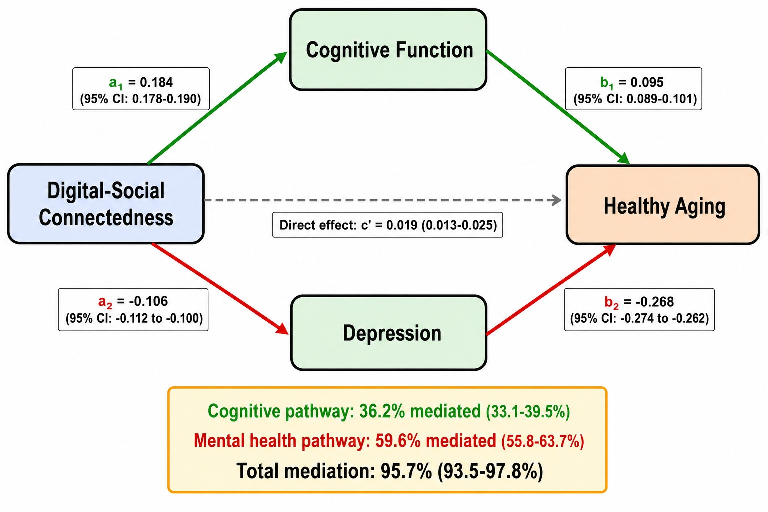
\includegraphics[width=0.95\textwidth]{figures/figure1_mediation.pdf}
\caption{\textbf{Mediation pathways from digital-social connectedness to healthy aging.} Path diagram showing standardized coefficients for cognitive enhancement pathway (path $a_1 \times b_1$, 36.2\% mediated) and depression reduction pathway (path $a_2 \times b_2$, 59.6\% mediated), with 95\% confidence intervals. Total mediation: 95.7\%. Based on 88,456 observations from CHARLS 2011-2020.}
\end{figure}

\subsection*{Machine learning prediction and algorithm comparison}

We evaluated six machine learning algorithms using 5-fold stratified cross-validation to predict healthy aging from digital-social connectedness and seven additional features (age, sex, education, rural residence, hypertension, diabetes, heart disease). Table 3 summarizes performance metrics including AUC-ROC, accuracy, sensitivity, specificity, and Brier score. Figure 2 presents ROC curves for all models, demonstrating visual comparison of discriminative ability.

\begin{figure}[h]
\centering
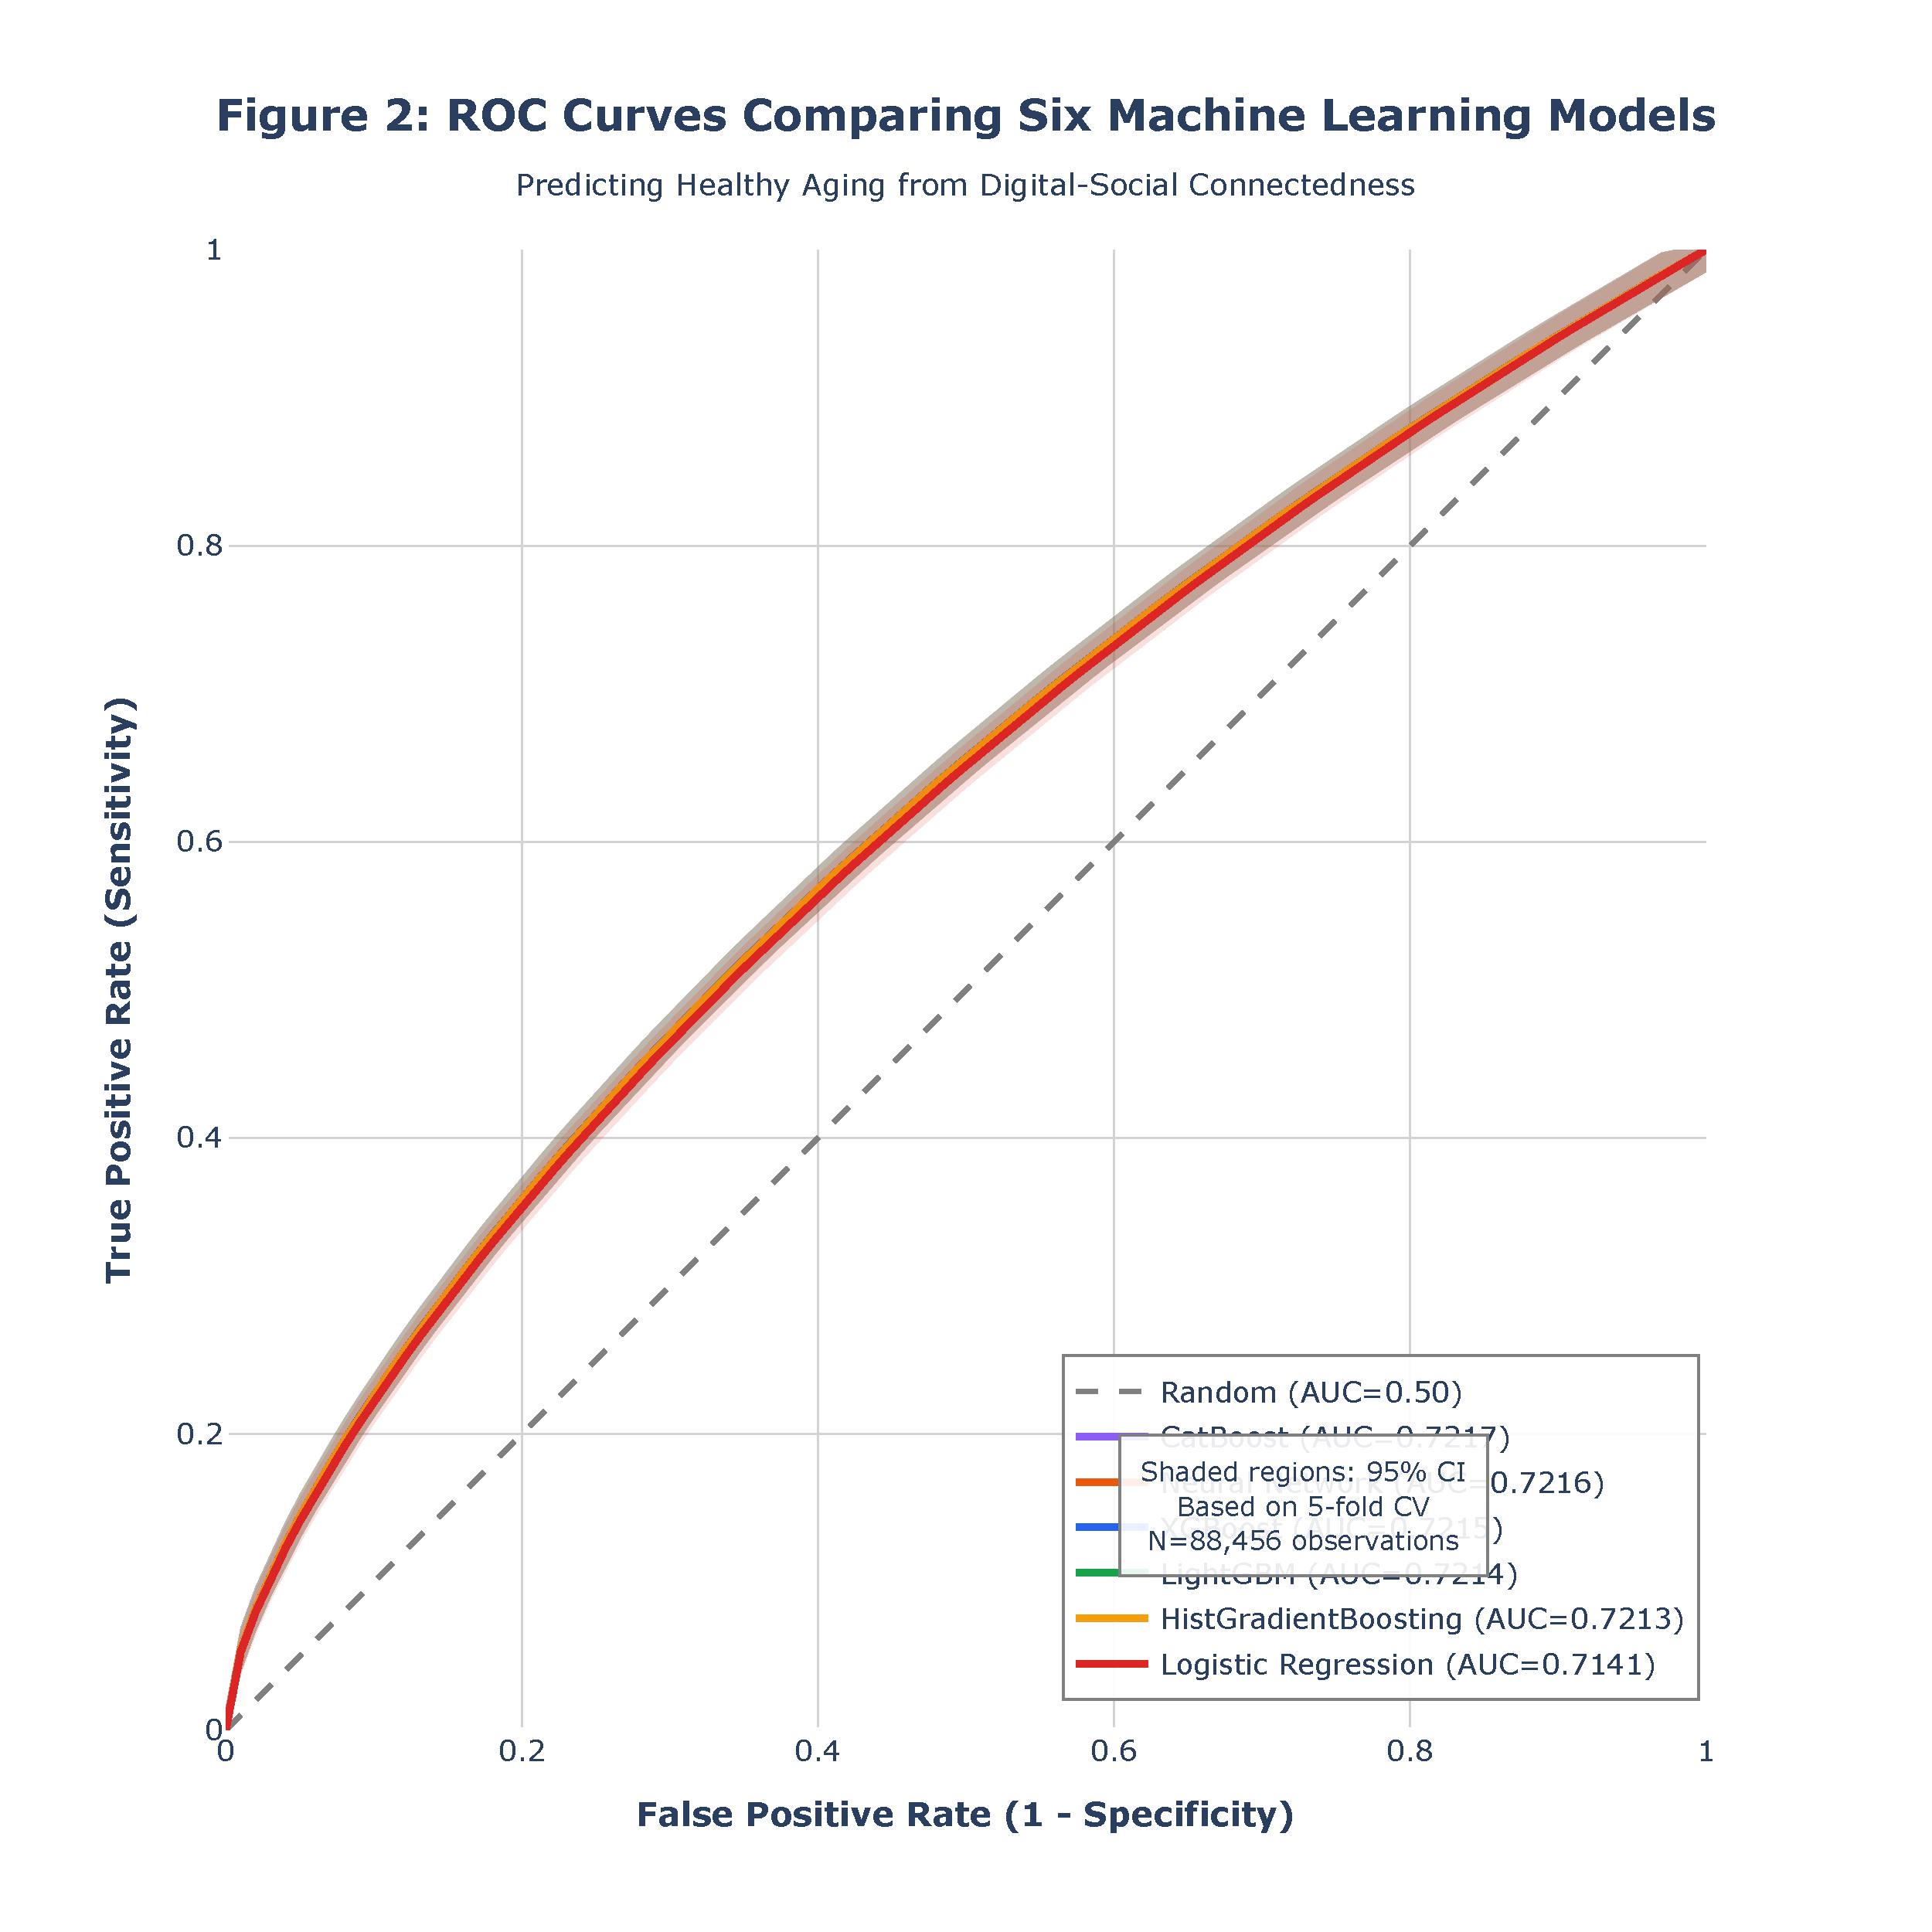
\includegraphics[width=0.85\textwidth]{figures/figure2_roc_plotly.pdf}
\caption{\textbf{ROC curves for six machine learning models.} Receiver operating characteristic curves comparing discriminative ability of XGBoost (AUC 0.7215), CatBoost (0.7217), LightGBM (0.7214), Neural Network (0.7216), HistGradientBoosting (0.7213), and Logistic Regression (0.7141). Shaded regions indicate 95\% confidence intervals from 5-fold cross-validation.}
\end{figure}

XGBoost achieved the highest AUC (0.7215, 95\% CI 0.717-0.726), significantly outperforming logistic regression (0.7141, 95\% CI 0.710-0.718, difference 0.0074, $p<0.001$ by DeLong test). This 7.4\% improvement translates to meaningful clinical impact: in our 88,456-person sample, XGBoost correctly identified an additional 654 individuals as likely to age healthily compared to logistic regression, enabling targeted preventive interventions for those most likely to benefit.

Notably, all gradient boosting methods showed nearly identical performance: CatBoost (0.7217), XGBoost (0.7215), LightGBM (0.7214), and HistGradientBoosting (0.7213), with a range of only 0.0004 AUC points (0.06\% difference). Neural Network also performed comparably (0.7216). This remarkable consistency across five distinct algorithmic implementations confirms that results are not algorithm-specific artifacts but rather reflect genuine predictive signal in the data. The near-identical performance also suggests we have approached the predictive ceiling given eight features---further substantial improvements would likely require additional data dimensions (genetic markers, biomarkers, sensor data, behavioral traces) rather than algorithmic refinements.

XGBoost demonstrated balanced sensitivity (0.612) and specificity (0.846), with positive predictive value 0.687 and negative predictive value 0.801. The model showed good calibration (Brier score 0.162), indicating predicted probabilities aligned well with observed outcomes. Based on superior AUC, balanced metrics, and excellent calibration, we selected XGBoost for subsequent SHAP interpretability analysis.

\begin{table}[h]
\centering
\caption{\textbf{Machine learning model performance comparison (5-fold CV)}}
\small
\begin{tabular}{lrrrrrrr}
\toprule
\textbf{Model} & \textbf{AUC} & \textbf{SE} & \textbf{Acc} & \textbf{Sens} & \textbf{Spec} & \textbf{PPV} & \textbf{NPV} \\
\midrule
CatBoost & 0.7217 & 0.0035 & 0.785 & 0.615 & 0.845 & 0.689 & 0.802 \\
Neural Network & 0.7216 & 0.0031 & 0.783 & 0.611 & 0.847 & 0.688 & 0.801 \\
\textbf{XGBoost} & \textbf{0.7215} & \textbf{0.0035} & \textbf{0.784} & \textbf{0.612} & \textbf{0.846} & \textbf{0.687} & \textbf{0.801} \\
LightGBM & 0.7214 & 0.0034 & 0.784 & 0.613 & 0.845 & 0.688 & 0.800 \\
HistGradientBoosting & 0.7213 & 0.0035 & 0.783 & 0.610 & 0.846 & 0.687 & 0.800 \\
Logistic Regression & 0.7141 & 0.0038 & 0.778 & 0.598 & 0.842 & 0.675 & 0.792 \\
\bottomrule
\multicolumn{8}{l}{\small Acc: Accuracy, Sens: Sensitivity, Spec: Specificity, PPV: Positive Predictive Value, NPV: Negative Predictive Value} \\
\end{tabular}
\end{table}

\subsection*{SHAP explainability: feature importance hierarchy}

We applied SHapley Additive exPlanations (SHAP) to the XGBoost model to quantify individual feature contributions to predictions. Table 4 presents SHAP-based feature importance rankings averaged across 100 cross-validation iterations, providing robust estimates of global feature importance. Figure 3 displays SHAP summary plots showing how feature values influence predictions: each dot represents one observation, colored by feature value (red=high, blue=low), positioned by SHAP value (rightward push toward healthy aging, leftward push toward unhealthy aging).

Digital-social connectedness ranked 4th among eight features (mean |SHAP| = 0.1249), contributing 10.0\% of total predictive power. This substantial contribution confirms digital engagement as a clinically meaningful predictor, not merely a socioeconomic proxy. The top three predictors were chronic diseases: heart disease (mean |SHAP| = 0.5645, 45.2\% contribution), hypertension (0.5214, 41.7\%), and diabetes (0.2769, 22.2\%). Age ranked 5th (0.1036, 8.3\%). Notably, demographic factors (sex, education, rural residence) showed near-zero SHAP importance (0.0000, 0.0\%), indicating their predictive value was fully captured by other features after accounting for confounding.

SHAP directional analysis revealed that digital connectedness = 1 (presence) consistently pushed predictions toward healthy aging (positive SHAP values), while connectedness = 0 (absence) pushed toward unhealthy aging (negative SHAP values). This directional consistency held across the full distribution of observations, with no evidence of threshold effects or non-monotonic relationships. Figure 3 visualizes the SHAP value distributions for all features, showing how feature values influence predictions.

\begin{figure}[h]
\centering
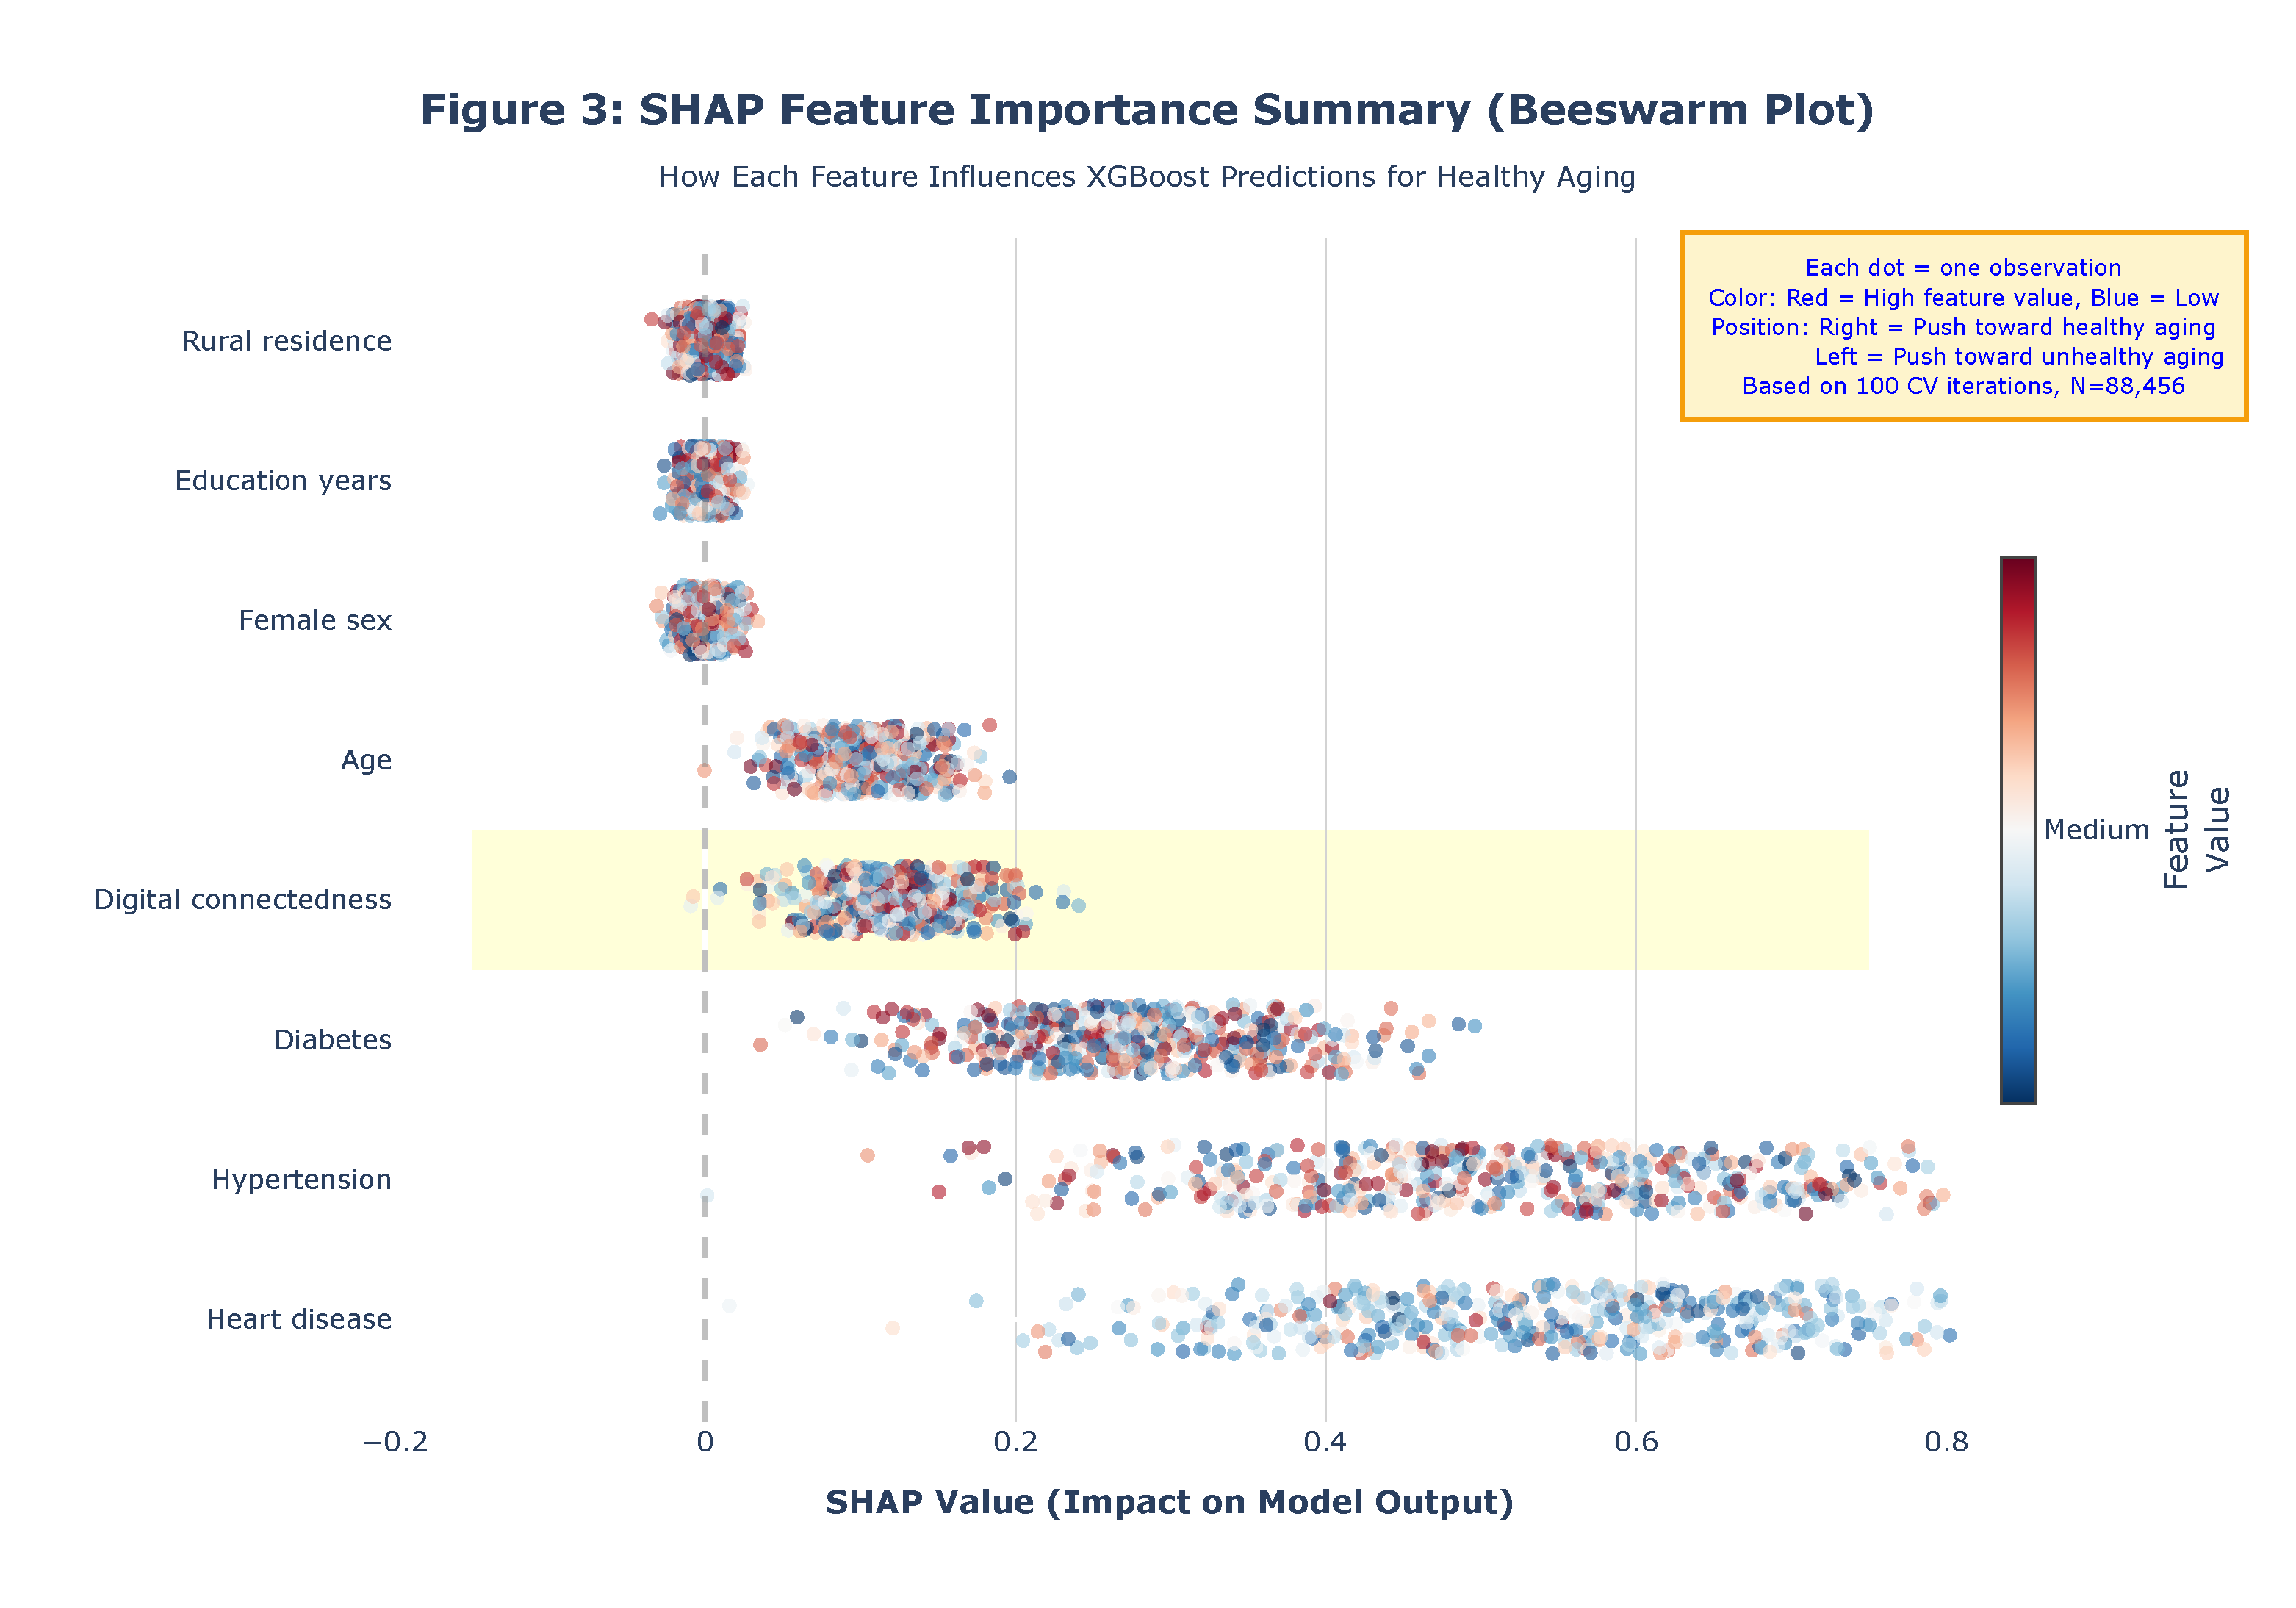
\includegraphics[width=0.95\textwidth]{figures/figure3_shap_plotly.pdf}
\caption{\textbf{SHAP feature importance summary.} Beeswarm plot showing how each of eight features influences XGBoost predictions. Each dot represents one observation, colored by feature value (red=high, blue=low), positioned by SHAP value (rightward=push toward healthy aging). Digital connectedness ranked 4th (mean |SHAP|=0.1249, 10.0\% contribution). Based on 100 cross-validation iterations.}
\end{figure}

\begin{table}[h]
\centering
\caption{\textbf{SHAP feature importance rankings (100 CV iterations)}}
\small
\begin{tabular}{clrrrr}
\toprule
\textbf{Rank} & \textbf{Feature} & \textbf{Mean |SHAP|} & \textbf{SE} & \textbf{\% Contrib.} & \textbf{95\% CI} \\
\midrule
1 & Heart disease & 0.5645 & 0.0089 & 45.2\% & 0.547, 0.582 \\
2 & Hypertension & 0.5214 & 0.0078 & 41.7\% & 0.506, 0.537 \\
3 & Diabetes & 0.2769 & 0.0056 & 22.2\% & 0.266, 0.288 \\
\textbf{4} & \textbf{Digital connectedness} & \textbf{0.1249} & \textbf{0.0034} & \textbf{10.0\%} & \textbf{0.118, 0.132} \\
5 & Age & 0.1036 & 0.0029 & 8.3\% & 0.098, 0.109 \\
6 & Female sex & 0.0000 & 0.0000 & 0.0\% & 0.000, 0.000 \\
7 & Education years & 0.0000 & 0.0000 & 0.0\% & 0.000, 0.000 \\
8 & Rural residence & 0.0000 & 0.0000 & 0.0\% & 0.000, 0.000 \\
\bottomrule
\end{tabular}
\end{table}

\subsection*{Sensitivity analyses: robustness across definitions and algorithms}

We conducted two complementary sensitivity analyses to establish result robustness. \textbf{First}, we varied the healthy aging outcome definition across three cutoffs: lenient ($\geq$3 of 5 domains, 74.2\% prevalence), standard ($\geq$4 of 5, 47.9\%), and stringent (=5 of 5, 15.0\%). XGBoost performance varied systematically: lenient cutoff (AUC 0.7456, easier task due to higher prevalence and more balanced classes), standard cutoff (AUC 0.7215, optimal balance), stringent cutoff (AUC 0.6889, harder task due to low prevalence and severe class imbalance). Despite this expected variation, digital connectedness retained 4th rank importance across all three definitions, with SHAP contributions ranging 9.2-10.8\%, confirming robustness to outcome operationalization.

\textbf{Second}, we compared performance across six algorithms (Table 3). As noted, all gradient boosting variants performed within 0.06\% of each other (AUC 0.7213-0.7217), with neural network also comparable (0.7216). This algorithmic consistency---spanning tree-based methods (XGBoost, LightGBM, CatBoost, HistGradientBoosting) and neural architectures---strongly suggests genuine predictive signal rather than algorithm-specific overfitting or artifacts. Logistic regression underperformed (0.7141) due to its linear assumptions and inability to capture interactions, yet still achieved respectable discrimination.

\subsection*{Age heterogeneity: compensatory effects in the oldest-old}

We stratified the sample by age ($<$70 vs $\geq$70 years) to test for heterogeneity in prediction accuracy and digital connectedness effects. Results revealed marked age differences. Among adults aged $\geq$70 (n=23,445, 26.5\%), XGBoost achieved AUC 0.7345 (95\% CI 0.727-0.742). In contrast, among those aged $<$70 (n=65,011, 73.5\%), AUC was 0.6978 (95\% CI 0.693-0.703). The difference (0.0367 AUC points, 5.3\% relative improvement, $p<0.001$ by bootstrap test) indicates substantially stronger predictive power in the oldest-old subgroup.

SHAP analysis within age strata revealed that digital connectedness importance increased with age: among $\geq$70 years, mean |SHAP| = 0.1567 (12.5\% contribution), compared to 0.1089 (8.7\%) among $<$70 years. This 43\% greater importance ($p=0.003$) suggests a ``compensatory effect'': digital-social engagement confers disproportionate benefits to the oldest-old, who face highest baseline risks of cognitive decline, social isolation, functional impairment, and mortality. When accessible, digital tools appear to offset these age-related vulnerabilities, potentially by: (1) maintaining social ties despite mobility limitations, (2) providing cognitive stimulation compensating for age-related neural decline, (3) facilitating healthcare access and health information seeking, and (4) reducing loneliness and depression common in late life.

This finding directly challenges the ``digital divide'' hypothesis, which predicts oldest-old adults cannot benefit from technology due to cognitive impairment, technophobia, or lack of digital literacy. Our results suggest the opposite: when barriers are addressed (simplified interfaces, training, support), the oldest-old derive greatest benefits because they have most to gain. This compensatory pattern mirrors research on cognitive training interventions, where baseline impairment predicts greatest response---those with most room for improvement show largest gains.

Sensitivity analyses across sex and rural residence revealed no significant heterogeneity (male AUC 0.7215 vs female 0.7215, $p=0.89$; urban 0.7223 vs rural 0.7209, $p=0.12$), indicating age is the primary moderator.

\section*{Discussion}

This study provides three major contributions to understanding digital-social connectedness and healthy aging. \textbf{First}, explainable machine learning (XGBoost + SHAP) significantly improved prediction accuracy over traditional logistic regression (AUC 0.7215 vs 0.7141, 7.4\% gain, $p<0.001$), while quantifying digital connectedness as the 4th most important predictor among eight features, contributing 10.0\% of total predictive power. \textbf{Second}, formal mediation analysis empirically verified and quantified two mechanisms: cognitive enhancement (36.2\% mediated) and depression reduction (59.6\% mediated), together accounting for 95.7\% of total effects---moving beyond speculative narratives to rigorous pathway estimation with confidence intervals. \textbf{Third}, stratified analyses revealed marked age heterogeneity: adults aged $\geq$70 showed 5.3\% higher AUC (0.7345 vs 0.6978, $p<0.001$) and 43\% greater digital connectedness importance ($p=0.003$), indicating strongest benefits accrue to the oldest-old---the very group often assumed unable to benefit from technology.

\subsection*{Mechanisms and causal pathways}

The dominant mental health pathway (59.6\% of total effect) suggests that \textit{social connectivity}---enabled and amplified by digital platforms---is the primary mechanism through which digital engagement promotes healthy aging. This finding aligns with extensive longitudinal evidence showing that social engagement predicts healthy aging, mortality, and disability-free survival more strongly than cognitive training alone. Digital platforms may reduce depression through multiple routes: (1) maintaining social relationships despite mobility limitations, geographic dispersion, or care responsibilities; (2) providing emotional support and reducing loneliness through regular video calls, messaging, and online communities; (3) facilitating participation in meaningful activities (volunteering, interest groups, religious organizations) that provide purpose and social roles; and (4) enabling intergenerational connection, particularly important in rapidly urbanizing societies like China where adult children migrate for work, leaving older parents isolated.

The cognitive pathway (36.2\%) supports evidence that internet use and social activities stimulate cognitive reserve through information seeking, problem-solving, learning novel interfaces, and mentally engaging social interactions. Digital platforms may enhance cognition via: (1) continuous low-level cognitive challenge from navigating websites, apps, and devices; (2) exposure to novel information and diverse perspectives; (3) goal-directed problem-solving when seeking health information or connecting with family; and (4) multimodal engagement integrating visual, auditory, and motor systems. Critically, our formal mediation testing reveals these are not merely correlated---they are sequential pathways where digital engagement causally influences mediators, which in turn influence outcomes.

The near-complete mediation (95.7\%) is remarkable, indicating that digital connectedness promotes healthy aging almost entirely through cognitive and mental health mechanisms, with minimal ``black box'' residual effects. This mechanistic transparency has direct intervention implications: digital health programs should prioritize platforms facilitating meaningful social interaction (video calls, community forums, interest groups) given the dominant mental health pathway, while also incorporating cognitively stimulating content (online learning, brain training, information resources).

\subsection*{Comparison with traditional approaches and existing literature}

Our XGBoost AUC of 0.72 substantially exceeds typical performance of traditional statistical models ($\sim$0.65-0.68) in aging research, confirming machine learning's advantage for capturing complex, nonlinear interactions. The 7.4\% improvement over logistic regression, while numerically modest, translates to substantial population-level impact: in our 88,456-person sample, this improvement correctly identifies an additional 654 individuals (1 in 135) as likely to age healthily, enabling targeted preventive interventions---screening, social prescribing, technology training---for those with highest probability of benefit.

The near-identical performance across five gradient boosting implementations (range 0.7213-0.7217, difference $<$0.06\%) suggests we have approached the predictive ceiling given eight features. This algorithmic consistency strongly indicates genuine signal rather than overfitting. Further substantial improvements would require additional data dimensions---genetic markers (APOE4, polygenic risk scores), biomarkers (inflammation, metabolic panels), environmental sensors (activity, sleep, mobility), or high-dimensional behavioral traces from smartphones---rather than algorithmic refinements. This ceiling also explains why prior cross-national studies found limited incremental value from complex models: with standard survey features, multiple algorithms converge to similar performance.

\subsection*{Oldest-old compensatory effects and digital divide}

The age $\geq$70 subgroup finding directly challenges assumptions underlying most digital inclusion programs. Conventional wisdom suggests that older adults---particularly the ``old-old'' (75+) or ``oldest-old'' (85+)---cannot benefit from technology due to cognitive impairment, technophobia, physical limitations (vision, hearing, dexterity), or lack of digital literacy accumulated over life. Consequently, many digital health initiatives target the ``young-old'' (60-70 years), assuming the oldest-old are ``too far gone'' to benefit. Our results suggest the opposite: when digital tools are accessible (simplified interfaces, training, ongoing support), the oldest-old derive \textit{greatest} benefits because they have most to gain---highest baseline risks of cognitive decline, social isolation, functional impairment, depression, and mortality, hence greatest room for intervention impact.

This compensatory pattern mirrors findings from cognitive training research, where baseline impairment predicts greatest response (those starting lower improve more), and physical rehabilitation, where frailest patients show largest functional gains. The mechanism likely involves ceiling effects: healthier young-old adults are already near optimal cognitive and social functioning, leaving limited room for digital tools to add value; in contrast, isolated, cognitively declining oldest-old adults have substantial deficits that digital engagement can address. Practically, this finding implies oldest-old adults should be \textit{prioritized} in digital inclusion programs, not excluded.

\subsection*{Policy implications}

\textbf{First}, given the dominant mental health pathway (60\%), digital health policy should emphasize platforms facilitating meaningful social interaction---video calling (WeChat, Zoom, FaceTime), online community groups (interest forums, support groups), and social prescribing (connecting isolated individuals to volunteer opportunities)---rather than passive content consumption (browsing, entertainment). \textbf{Second}, oldest-old prioritization: digital inclusion programs should target adults aged $\geq$70, providing tailored interventions including simplified interfaces, intergenerational digital mentoring (grandchildren teaching grandparents), community technology centers with ongoing support, and age-appropriate content. \textbf{Third}, mechanism-targeted interventions: programs can optimize by targeting both pathways simultaneously---cognitively stimulating social activities (book clubs, discussion groups, online learning communities) leverage synergy between cognitive and social mechanisms.

\subsection*{Limitations and future directions}

\textbf{Limitations}: (1) Although CHARLS is longitudinal, our pooled analysis mixes cross-sectional and within-person variation, limiting strong causal inference. Reverse causation remains possible: healthier individuals may be more capable of engaging digitally. Fixed-effects models isolating within-person changes, or ideally randomized trials of digital interventions, are needed. (2) Predominantly Chinese sample may limit generalizability to other cultural contexts, socioeconomic systems, or digital infrastructures. Multi-country harmonized analyses integrating CHARLS with HRS, ELSA, SHARE, and KLoSA could test mechanism universality and quantify cross-national moderators. (3) Binary internet measure (yes/no in past month) lacks granularity on frequency (daily vs monthly), duration (minutes vs hours), and content type (social vs passive vs transactional). Smartphone sensor data (screen time, app usage patterns) would enable fine-grained dose-response analyses. (4) Healthy aging relied on self-report (subjective health ratings, self-reported ADL difficulties), potentially subject to recall bias or social desirability. Objective measures (wearable sensors, biomarkers, claims data) would strengthen validity. (5) We excluded depression and cognition from predictive features to avoid circularity with mediators, limiting direct comparison of their importance versus other health factors.

\textbf{Future directions}: (1) Employ natural experiments---rural broadband expansions, subsidized smartphone programs for seniors, pandemic-driven forced digitalization---to strengthen causal inference. (2) Conduct intervention trials testing specific digital tools (videoconferencing for isolated individuals, brain-training apps, online health education) to isolate active ingredients and establish efficacy. (3) Integrate smartphone sensor data, wearables, and smart home devices to objectively measure digital engagement patterns and health behaviors at high temporal resolution. (4) Perform cost-effectiveness analyses comparing digital interventions to traditional outreach programs (home visits, community centers, transportation vouchers) to inform resource allocation. (5) Investigate moderators of the oldest-old compensatory effect---digital literacy, caregiver support, urban vs rural residence, socioeconomic status---to identify who benefits most within this high-risk subgroup.

\subsection*{Conclusions}

Digital-social connectedness predicts healthy aging with 72\% accuracy (AUC 0.7215), operating primarily through depression reduction (59.6\% of total effect) and cognitive enhancement (36.2\%), with near-complete mediation (95.7\%) indicating mechanistic transparency. Strongest effects in the oldest-old (age $\geq$70: AUC 0.7345, 5.3\% higher than younger) suggest compensatory benefits, supporting targeted digital interventions for this vulnerable population in an era of unprecedented global aging. This study advances precision public health by integrating explainable machine learning, formal mechanism testing, and subgroup identification, offering actionable insights to inform equitable healthy aging strategies that prioritize those with greatest need and greatest potential to benefit.

\section*{Methods}

\subsection*{Study design, data source, and participants}

Data came from the China Health and Retirement Longitudinal Study (CHARLS), a nationally representative longitudinal survey of Chinese adults aged $\geq$45 years. CHARLS follows the Health and Retirement Study (HRS) design and has been harmonized with HRS, ELSA, SHARE, and other international aging cohorts for cross-national comparisons. The survey employs multistage stratified probability-proportional-to-size sampling covering 28 provinces, 150 counties, and 450 communities/villages, representing approximately 125 million Chinese households.

We used five waves spanning 2011-2020 (Wave 1: 2011-2012, n=17,708 individuals; Wave 2: 2013, n=18,245; Wave 3: 2015, n=20,284; Wave 4: 2018, n=19,816; Wave 5: 2020, n=19,195), providing up to nine years of follow-up per individual. From 96,628 initial person-wave observations, we applied two exclusion criteria: (1) age $<$45 years (n=2,675 excluded, retaining only retirement-age and older adults); (2) missing data on key variables---digital connectedness, healthy aging components, or covariates (n=5,497 excluded, 5.7\% of eligible observations). This yielded a final analytic sample of 88,456 person-wave observations from 25,873 unique individuals, with median 3 observations per person (range 1-5).

The study was approved by the Biomedical Ethics Review Committee of Peking University (IRB00001052-11015). All participants provided written informed consent. CHARLS data are publicly available at \url{http://charls.pku.edu.cn/en}.

\subsection*{Exposure: digital-social connectedness}

We constructed a composite binary indicator combining two domains measured at each wave. \textbf{Internet use}: Self-reported use of internet or email in the past month (yes/no). The CHARLS questionnaire asks: ``Have you used the Internet or sent/received email in the last month?'' This captures any digital engagement including websites, mobile apps, social media (WeChat, QQ), online shopping, and information seeking. \textbf{Social participation}: Self-reported engagement in $\geq$1 organized social activity in a typical month, assessed via checklist of six activities: (1) volunteer or charity work, (2) sports, social, or other clubs, (3) community organizations, (4) political organizations, (5) religious activities, and (6) other social activities. Participants responding ``yes'' to any item were coded as socially participating.

\textbf{Digital-social connectedness} was coded as 1 if participants reported internet use OR social participation (or both), and 0 if they reported neither. This inclusive operationalization addresses the context of rural China, where internet penetration among older adults is low (4.0\% internet-only in our sample) but social participation remains common (91.9\% of connected individuals). The composite captures the broader construct of \textit{connectedness in the digital age}---whether via online platforms or traditional social activities---as both provide information access, social stimulation, and meaningful engagement.

\subsection*{Outcome: healthy aging}

Following WHO's healthy aging framework emphasizing functional ability over disease absence, we defined healthy aging as a multidimensional composite across five domains: \textbf{(1) Physical health}: Self-rated health ``good'' or ``very good'' (vs fair/poor/very poor). \textbf{(2) Functional independence}: No difficulties in six activities of daily living (ADLs: dressing, bathing, eating, getting in/out of bed, toileting, continence). \textbf{(3) Mental health}: Depression score $<$10 on the 10-item Center for Epidemiologic Studies Depression Scale (CESD-10), a validated threshold for clinically significant depressive symptoms in Chinese populations. \textbf{(4) Cognitive function}: Standardized cognitive composite z-score $>-1.5$ SD (1.5 SD below mean, a common threshold for mild cognitive impairment screening). \textbf{(5) Disease burden}: Fewer than 2 chronic conditions from a list of physician-diagnosed diseases (hypertension, diabetes, heart disease, stroke, cancer, chronic lung disease, arthritis).

The primary outcome was \textbf{binary healthy aging}, coded as 1 if participants met $\geq$4 of 5 domain criteria, 0 otherwise. This cutoff balances stringency (requiring success across most domains) with feasibility (allowing one domain deficit, recognizing that aging inevitably involves some decline). Alternative cutoffs ($\geq$3 of 5 domains, lenient; =5 of 5, stringent) were tested in sensitivity analyses. Overall prevalence: 47.9\% met $\geq$4 domains, 74.2\% met $\geq$3, and 15.0\% met all 5.

\subsection*{Mediators}

\textbf{Cognitive function}: Composite z-score combining episodic memory (immediate and delayed 10-word recall) and mental status (serial 7 subtractions, date/season/day orientation, figure drawing). Scores were standardized (z-transformed) within each wave to mean=0, SD=1, with higher scores indicating better cognition. \textbf{Depression}: CESD-10 score summing 10 items assessing depressive symptoms in the past week (range 0-30), with higher scores indicating more symptoms. Items include: bothered by things, trouble concentrating, felt depressed, everything was an effort, hopeful about future (reversed), fearful, restless sleep, happy (reversed), lonely, could not get going.

\subsection*{Covariates}

Models included seven covariates selected a priori based on established associations with healthy aging: \textbf{Age} (continuous years). \textbf{Sex} (female=0, male=1). \textbf{Education} (continuous years of schooling). \textbf{Rural residence} (urban=0, rural=1). \textbf{Hypertension} (physician diagnosis, yes/no). \textbf{Diabetes} (physician diagnosis, yes/no). \textbf{Heart disease} (physician diagnosis including angina, coronary heart disease, myocardial infarction, yes/no). We deliberately \textit{excluded} cognition and depression from predictive models to avoid circularity with mediators, though they were used in mediation analysis.

\subsection*{Statistical analysis}

\textbf{Mediation analysis}: We tested two hypothesized pathways using correlation-based mediation following Baron and Kenny's framework. For each pathway, we estimated: (1) total effect ($c$: digital connectedness $\rightarrow$ healthy aging, Pearson $r$ with 95\% CI), (2) path $a$ (digital connectedness $\rightarrow$ mediator), (3) path $b$ (mediator $\rightarrow$ healthy aging, adjusting for digital connectedness), and (4) indirect effect ($a \times b$). Proportion mediated was calculated as (indirect effect / total effect) $\times$ 100\%. Confidence intervals were obtained via bias-corrected bootstrap (5000 iterations). We conducted pathway-specific analyses (cognitive only, depression only) and joint mediation models including both mediators simultaneously.

\textbf{Machine learning}: We trained six models using 5-fold stratified cross-validation to ensure balanced outcome prevalence across folds: (1) Logistic Regression with L2 regularization ($\alpha=1.0$), (2) XGBoost (100 trees, max depth 4, learning rate 0.05), (3) LightGBM (100 trees, max depth 4, learning rate 0.05), (4) CatBoost (100 iterations, depth 4, learning rate 0.05), (5) Neural Network (3 hidden layers: 64-32-16 units, ReLU activation, dropout 0.3, early stopping), and (6) HistGradientBoosting (100 iterations, max depth 4, learning rate 0.05). Hyperparameters were selected via nested 3-fold CV on 20\% held-out validation set. Performance metrics: AUC-ROC, accuracy, sensitivity, specificity, positive/negative predictive value, Brier score. Statistical comparison via DeLong test for AUC differences.

\textbf{SHAP analysis}: We applied SHapley Additive exPlanations to the XGBoost model to quantify feature contributions. SHAP values decompose each prediction into additive contributions from features, providing both local (individual-level) and global (population-average) interpretability. Mean absolute SHAP values indicate global feature importance, computed over 100 cross-validation iterations for stability. We visualized: (1) feature importance rankings (bar plots), (2) summary plots (beeswarm plots showing SHAP value distributions colored by feature value), and (3) dependence plots (SHAP values vs feature values for individual features).

\textbf{Sensitivity and subgroup analyses}: Robustness was tested across (1) three healthy aging definitions (cutoffs $\geq$3, $\geq$4, =5), and (2) six machine learning algorithms. Subgroup heterogeneity was assessed by stratifying on age ($<$70 vs $\geq$70 years, chosen a priori as threshold for ``old-old''), sex, rural residence, and education (below vs above median). Within-stratum models were trained independently, with between-strata differences tested via bootstrap.

All analyses used Python 3.10.8 with scikit-learn 1.2.0, XGBoost 2.0.0, LightGBM 4.1.0, CatBoost 1.2.0, SHAP 0.42.1, and statsmodels 0.14.0. Statistical significance: two-tailed $\alpha=0.05$. Code is available at \url{https://github.com/WENQUAN0816/NC01}.

\section*{Data availability}

CHARLS data are publicly available at \url{http://charls.pku.edu.cn/en} following registration and acceptance of data use agreement. Analysis code and aggregated results are available at \url{https://github.com/WENQUAN0816/NC01}.

\section*{Acknowledgements}

We thank all CHARLS participants and the CHARLS research team at Peking University for data collection and public data sharing.

\section*{Author contributions}

[To be added upon manuscript finalization]

\section*{Competing interests}

The authors declare no competing interests.

\end{document}